\section{Udvælgelse af skalaer}
\label{ParametreDatabehandlingSkalaer}
%
Ud fra de fundne parametre og de potentielle skala spørgsmål beskrevet i forrige afsnit vil der i dette afsnit fokuseres på at udvælge de skalaer, der fremadrette vil blive anvendt i forbindelse med at evaluere interaktionen med robotten. I det henseende kan det være at to eller flere tidligere foreslået skala spørgsmål bliver sammensat til ét i tilfælde af, at det vurderes, at de vedrører den samme parameter. Denne vurdering foretages blandt projektgruppen, hvorfor der er ikke er fastsatte kriterier for hvornår to skala spørgsmål sammensættes, udover at de vedrører det samme.

Et krav for udvælgelsen af et skala spørgsmål er, at det skal være muligt at ændre på den specifikke parameter. Derudover vil de udvalgte skala spørgsmål blive præsenteret på deres respektive skalaer. Det tilstræbes at opstille den optimale skala for hvert enkelt parameter, hvorfor der ikke er fastsat én specifik skala type på forhånd.\blankline
%
I henhold til den første kategori: \textit{Interagerer ikke med R}, hvor der kun er ét potentielt skala spørgsmål: \textit{Er det let at undgå R}, så vil dette skala spørgsmål ikke fremgå på en endelig skala. Årsagen er, at spørgsmålet vil blive sammensæt med: \textit{Jeg synes at robotten er anmassende}. Vurderingen bygger på, at hvis robotten er anmassende vil den formentlig ikke være let at undgå, hvorimod hvis robotten slet ikke er anmassende så er robotten formentlig let at undgå. 

Skala spørgsmålet: \textit{Hvordan synes du skærmen virkede}, vil ikke behandles på lige fod med de resterende parametre, men det kan være med til at undersøge hvorvidt skærmens reaktionsevne har en indflydelse på interaktionen. Grunden til at spørgsmålet ikke vil indgå på samme måde som de resterende parametre er, at det forventes at den færdig udviklede robot ikke vil have dette problem. Problemet med at skærmen reagerer dårligt skyldes formentlig, at \textit{wireframet} åbnes igennem robottens egen software. Derudover er det observeret at flere testpersoner har problemer med at trykke på skærmen, hvor teorien/hypotesen er, at de trykker for hårdt. På \autoref{fig:SkalaSkaermensReaktion} fremgår skalaen, hvorpå det vurderes hvordan skærmen reagerede.  
%
\begin{figure}[H]
\centering
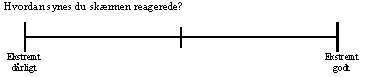
\includegraphics[width =\textwidth]{Figure/UdvalgteSkalaer/SkaermensReaktion} 
\caption{Bipolær VAS med lukkede endepunkter og unavngivet midtpunkt til skala spørgsmålet: \textit{Hvordan synes du skærmen reagerede?}}
\label{fig:SkalaSkaermensReaktion}
\end{figure}
\noindent
%
Årsagen til at der ikke er et label på midtpunktet på \autoref{fig:SkalaSkaermensReaktion} er, at det forventes, at der en logisk forståelse for hvad midten indikerer, hvor et label potentielt kan skævvride responsen. De to potentielle skala spørgsmål: \textit{Jeg føler at R kan hjælpe mig} og \textit{R kan hjælpe mig så jeg ikke behøver at spørger personale} bliver sammensat fordi de begge vedrører at robotten kan hjælpe dem. På \autoref{fig:SkalaRKanHjaelpe} fremgår den udvalgte skala for hvorvidt robotten kan hjælpe én.
%
\begin{figure}[H]
\centering
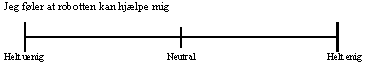
\includegraphics[width =\textwidth]{Figure/UdvalgteSkalaer/RobottenKanHjaelpe} 
\caption{Bipolær VAS med lukkede endepunkter og navngivet midtpunkt til skala spørgsmålet: \textit{Jeg føler at robotten kan hjælpe mig}.}
\label{fig:SkalaRKanHjaelpe}
\end{figure}
\noindent
%
Årsagen til at der på \autoref{fig:SkalaRKanHjaelpe} fremgår et label på midtpunktet er for, at kalibrer skalaen omkring neutral i tilfælde af, at testpersonen ikke har en holdning om hvorvidt robotten kan hjælpe en. Fra samme kategori: \textit{R kan assistere mennesker} udvælges skala spørgsmålet: \textit{Jeg oplever robottens hjælp som personlig}, hvilket fremgår på \autoref{fig:SkalaPersonligHjaelp}.
%
\begin{figure}[H]
\centering
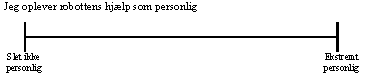
\includegraphics[width =\textwidth]{Figure/UdvalgteSkalaer/PersonligHjaelp} 
\caption{Unipolær VAS med lukkede endepunkter til skala spørgsmålet: \textit{Jeg oplever robottens hjælp som personlig}.}
\label{fig:SkalaPersonligHjaelp}
\end{figure}
\noindent
%
Årsagen til at skala spørgsmålet: \textit{Jeg oplever robottens hjælp som personlig} ikke præsenteres på en bipolær skala skyldes hovedsageligt, at der ikke findes en naturlig og logisk modpart til personlig. \textbf{Hvorfor bruger vi egentlig ikke "ekstremt upersonlig"?}.\blankline
%
I henhold til kategorien: \textit{R's væremåde} vil skala spørgsmålene vedrørende robottens bevægelse, hastighed samt hvorvidt robotten er irriterende vælges, som de fremgår i \fullref{ParametreRsVaeremaade}. Skalaen tilhørende robottens bevægelse fremgår på \autoref{fig:SkalaBevaegelserR}, robottens hastighed fremgår på \autoref{fig:SkalaHastighedR} og hvorvidt robotten er irriterende fremgår på \autoref{fig:SkalaIrriterende}.  
%
\begin{figure}[H]
\centering
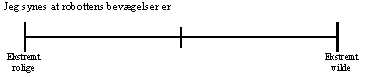
\includegraphics[width =\textwidth]{Figure/UdvalgteSkalaer/BevaegelserR} 
\caption{Bipolær VAS med lukkede endepunkter og unavngivet midtpunkt til skala spørgsmålet: \textit{Jeg synes at robottens bevægelser er}.}
\label{fig:SkalaBevaegelserR}
\end{figure}
\noindent
%
Årsagen til at \autoref{fig:SkalaBevaegelserR} er bipolær er, at det vurderes at ekstremt rolige bevægelser er det modsatte af ekstremt vilde bevægelser. Hvor årsagen til at der ikke er et label på midtpunktet er, at det vurderes, at der er en logisk adskilles mellem de to yderpunkter. Derudover er det svært at finde et label, som ville kunne kobles til midtpunktet mellem rolige og vilde bevægelser.
%
\begin{figure}[H]
\centering
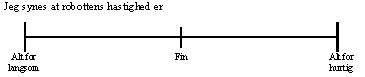
\includegraphics[width =\textwidth]{Figure/UdvalgteSkalaer/HastighedR} 
\caption{Bipolær VAS med lukkede endepunkter og navngivet midtpunkt til skala spørgsmålet: \textit{Jeg synes at robottens hastighed er}.}
\label{fig:SkalaHastighedR}
\end{figure}
\noindent
%
Årsagen til at \autoref{fig:SkalaHastighedR} præsenteres på en bipolær skala er, at de to labels på endepunkterne gengiver testpersonernes egne formulering af robottens hastighed. Derudover er midtpunkt angivet med: \textit{Fin}, fordi det afspejler testpersonernes udsagn. Ydermere vurderes det, at der ikke findes en naturlig og logisk midte mellem de to yderpunkter, hvorfor der kalibreres omkring at robottens hastighed er fin. 
%
\begin{figure}[H]
\centering
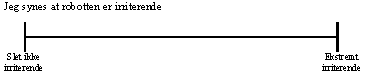
\includegraphics[width =\textwidth]{Figure/UdvalgteSkalaer/Irriterende} 
\caption{Unipolær VAS med lukkede endepunkter til skala spørgsmålet: \textit{Jeg synes at robotten er irriterende}.}
\label{fig:SkalaIrriterende}
\end{figure}
\noindent
%
Årsagen til at \autoref{fig:SkalaIrriterende} præsenteres på en unipolær skala er, at det vurderes, at der ikke forekommer en naturlig og logisk modpart til irriterende.

Derudover vælges det at sammensætte: \textit{Jeg synes at R er levende} fra kategori: \textit{R's væremåde} og \textit{Jeg synes at R ser menneskelig ud} fra kategori: \textit{R's udseende}, til ét enkelt skala spørgsmål præsenteret på \autoref{fig:SkalaMenneskeligR}.
%
\begin{figure}[H]
\centering
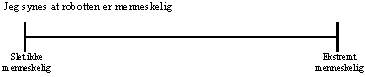
\includegraphics[width =\textwidth]{Figure/UdvalgteSkalaer/MenneskeligR} 
\caption{Unipolær VAS med lukkede endepunkter til skala spørgsmålet: \textit{Jeg synes at robotten er menneskelig}.}
\label{fig:SkalaMenneskeligR}
\end{figure}
\noindent
%
Årsagen til at \autoref{fig:SkalaMenneskeligR} præsenteres på en unipolær skala fremfor en bipolær skala er, at der ikke umiddelbart findes en naturlig og logisk modpart til menneskelig, hvertfald i forhold til robotten. Der kan argumenteres for, at anvende ordet: \textit{Umenneskelig}, hvor årsagen til at dette ord ikke anvendes er, at hvis en robot er umenneskelig er det så en maskine eller et dødt objekt, og i så fald hvilket ord skal da anvendes som label. På baggrund af dette blev det besluttet at angive modparten som: \textit{Slet ikke menneskelig}.

Ydermere sammensættes: \textit{Jeg synes at R er anmassende} fra kategori: \textit{R's væremåde}, med \textit{Jeg synes at R er intimiderende} fra kategori: \textit{Henvendelse}, samt \textit{Er det let at undgå R} fra kategori: \textit{Interagerer ikke med R}. Årsagen til at \textit{Jeg synes at R er intimiderende} sammensættes med hvorhvidt robotten er anmassende er, at vurderes at hvis robotten perciperes som værende ekstremt anmassende vil den formentlig også blive perciperet som intimiderende, hvorhvis robotten ikke er anmassende så forventes det ligeledes at robotten heller ikke perciperes som intimiderende. Årsagen til at \textit{Er det let at undgå R} indgår er forklaret tidligere. Den valgte skala fremgår på \autoref{fig:SkalaAnmassende}.  
%
\begin{figure}[H]
\centering
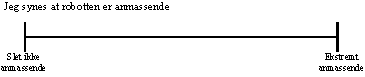
\includegraphics[width =\textwidth]{Figure/UdvalgteSkalaer/Anmassende} 
\caption{Unipolær VAS med lukkede endepunkter til skala spørgsmålet: \textit{Jeg synes at robotten er anmassende}.}
\label{fig:SkalaAnmassende}
\end{figure}
\noindent
%
Årsagen til at \autoref{fig:SkalaAnmassende} ikke præsenteres på en bipolær skala er, at det igen vurderes, at der ikke forekommer en naturlig og logisk modpart til anmassende. Af de fem potentielle skala spørgsmål fra kategorien: \textit{Henvendelse} er det kun \textit{Jeg synes at R er intimiderende}, der er blevet sammensat med et andet parametre. De fire resterende potentielle skala spørgsmål vælges derfor, hvilket fremgår af følgende figurer.    
%
\begin{figure}[H]
\centering
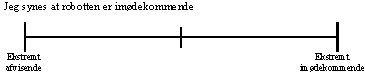
\includegraphics[width =\textwidth]{Figure/UdvalgteSkalaer/Imoedekommende} 
\caption{Bipolær VAS med lukkede endepunkter og unavngivet midtpunkt til skala spørgsmålet: \textit{Jeg synes at robotten er imødekommende}.}
\label{fig:SkalaImoedekommende}
\end{figure}
\noindent
%
Årsagen til at der ikke er et label på midtpunktet på \autoref{fig:SkalaImoedekommende} er, at det vurderes at midtpunktet i sig selv naturligt og logisk indikerer midten. Derudover har det ikke været muligt at finde et pasende ord, som kunne anvendes som label til midtpunktet.  
%
\begin{figure}[H]
\centering
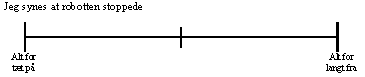
\includegraphics[width =\textwidth]{Figure/UdvalgteSkalaer/RStoppede} 
\caption{Bipolær VAS med lukkede endepunkter og unavngivet midtpunkt til skala spørgsmålet: \textit{Jeg synes at robotten stoppede}.}
\label{fig:SkalaRStoppede}
\end{figure}
\noindent
%
De to labels på henholdvist venstre og højre endepunkt, jævnfør \autoref{fig:SkalaRStoppede}, afspejler testpersonernes egne udsagn, hvor årsagen til at der ikke er et label på midtpunktet er den samme som ved den foregående skala. 
%
\begin{figure}[H]
\centering
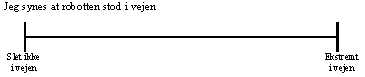
\includegraphics[width =\textwidth]{Figure/UdvalgteSkalaer/RobottenErIVejen} 
\caption{Unipolær VAS med lukkede endepunkter til skala spørgsmålet: \textit{Jeg synes at robotten stod i vejen}.}
\label{fig:SkalaRerIVejen}
\end{figure}
\noindent
%
Årsagen til at skalaen på \autoref{fig:SkalaRerIVejen} ikke præsenteres på en bipolær skala er, at det ikke har været muligt at angive en direkte modpart til at stå i vejen. 
%
\begin{figure}[H]
\centering
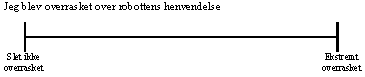
\includegraphics[width =\textwidth]{Figure/UdvalgteSkalaer/OverrasketOverR} 
\caption{Unipolær VAS med lukkede endepunkter til skala spørgsmålet: \textit{Jeg blev overrasket over robottens henvendelse}.}
\label{fig:SkalaOverrasketOverR}
\end{figure}
\noindent
%
Af samme årsag som før præsenteres skalaen på \autoref{fig:SkalaOverrasketOverR} på en unipolær skala. \blankline
%
I forhold til kategorien: \textit{R's udseende} besluttes det, at ekskludere det potentielle skala spørgsmål: \textit{Jeg kan godt lide R's udseende}, fordi det formentlig er en form for overkategori til de resterende parametre. Det forventes at i tilfælde af, at en testperson vurderer robotten som værende elegant, fra samme kategori, sød, sjov og sej, som kommer fra kategori: \textit{Positiv overfor R}, så vil en vurdering på hvor godt testpersonen kan lide robottens udseende ligeledes være positivt. Det antages derfor at hvorvidt danske rejsende kan lide robottens udseende måles indirekte ved de andre parametre, der omhandler robottens udseende.
%
\begin{figure}[H]
\centering
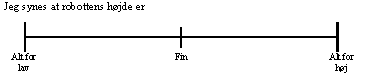
\includegraphics[width =\textwidth]{Figure/UdvalgteSkalaer/HoejdeR} 
\caption{Bipolær VAS med lukkede endepunkter med navngivet midtpunkt til skala spørgsmålet: \textit{Jeg synes at robottens højde er}.}
\label{fig:SkalaHoejdeR}
\end{figure}
\noindent
%
Årsagen til at robottens højde bliver evalueret på en bipolær skala, som illustreret på \autoref{fig:SkalaHoejdeR}, er, at høj og lav er modsætninger. At midtpunktet er navngivet: \textit{Fin} er baseret på testpersonernes egen oplevelse af robottens højde. Derudover kan det være med til at kalibrere de næste testpersonernes evaluering af robottens højde i forhold til skalaen. En anden årsag til at \textit{Fin} anvendes er, at der ikke nødvendigvis er en logisk højde lige akkurat mellem lav og høj. I dette tilfælde afspejler \textit{Fin} en højde, der svarer til omkring albuehøjde, som er den højde testpersonerne gav udtryk for var fin. 
%
\begin{figure}[H]
\centering
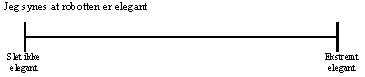
\includegraphics[width =\textwidth]{Figure/UdvalgteSkalaer/ElegantR} 
\caption{Unipolær VAS med lukkede endepunkter til skala spørgsmålet: \textit{Jeg synes at robotten er elegant}.}
\label{fig:SkalaElegantR}
\end{figure}
\noindent
%
Af samme årsag som tidligere, har det ikke været muligt at finde en naturlig og logisk modpart til \textit{elegant}, hvorfor denne skala præsenteres på en unipolær VAS, som fremgår af \autoref{fig:SkalaElegantR}.\blankline
%
Baseret på kategorien: \textit{Interesse for R} fremgår der to potentielle skala spørgsmål, som relaterer sig til hvorvidt robotten fangede ens opmærksomhed og om robotten er spændende, jævnfør \fullref{ParametreInteresseForR}. Det vælges at sammensætte de to potentielle skala spørgsmål til ét fordi det vurderes, at de relaterer til den samme oplevelse, da de begge tilhører den samme kategori. På \autoref{fig:SkalaRerSpaendende} fremgår skalaen udviklet til skala spørgsmålet: \textit{Jeg synes at robotten er spændende}. Det antages derfor at i tilfælde, hvor en testperson synes, at robotten er spændende så vil robotten ligeledes have fanget testpersonens opmærksomhed, hvorhvis testpersonen ikke synes, at robotten er spændende så er det ikke sikkert at den fanger ens opmærksomhed. Dertil kan der ligeledes opstå en situation, hvor robotten fanger en testpersons opmærksomhed uden, at testpersonen finder robotten spændende.
%
\begin{figure}[H]
\centering
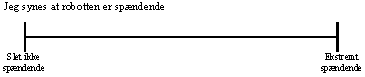
\includegraphics[width =\textwidth]{Figure/UdvalgteSkalaer/RerSpaendende} 
\caption{Unipolær VAS med lukkede endepunkter til skala spørgsmålet: \textit{Jeg synes at robotten er spændende}.}
\label{fig:SkalaRerSpaendende}
\end{figure}
\noindent
%
Igen har det hverken været muligt at finde en naturlig og logisk modpart til \textit{spændende} eller finde et label til et potentielt midtpunkt i tilfælde af, at der fandtes en modpart.\blankline 
%
Det vælges at medtage samtlige fire potentielle skala spørgsmål fra kategorien: \textit{Positiv overfor R}, jævnfør \autoref{ParametrePositivOverforR}. Robotten evalueres derfor i forhold til hvor sød, \autoref{fig:SkalaSoedR}, sjov, \autoref{fig:SkalaSjovR}, sej, \autoref{fig:SkalaSejR}, samt hvorvidt testpersonen kan lide at blive betjent af robotten, \autoref{fig:SkalaBetjeningAfR}. Årsagen til at de alle medtages er, at det forventes at de har en indflydelse på evalueringen af andre parametre. Derudover er \textit{sød}, \textit{sjov} og \textit{sej} parametre, som går igen ved flere testpersoner. 
%
\begin{figure}[H]
\centering
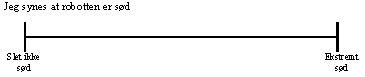
\includegraphics[width =\textwidth]{Figure/UdvalgteSkalaer/SoedR} 
\caption{Unipolær VAS med lukkede endepunkter til skala spørgsmålet: \textit{Jeg synes at robotten er sød}.}
\label{fig:SkalaSoedR}
\end{figure}
\noindent
%
Da det ikke med sikkerhed kan fastslåes, hvad testpersonerne har ment, da de gav udtryk for, at robotten er sød, har det ikke været mulig at finde en modpart. Det lader nemlig ikke til, at testpersonerne har brugt ordet \textit{sød} om robotten, hvor modsætningen da har været \textit{dum}.   
%
\begin{figure}[H]
\centering
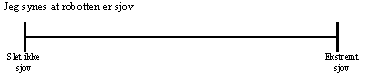
\includegraphics[width =\textwidth]{Figure/UdvalgteSkalaer/SjovR} 
\caption{Unipolær VAS med lukkede endepunkter til skala spørgsmålet: \textit{Jeg synes at robotten er sjov}.}
\label{fig:SkalaSjovR}
\end{figure}
\noindent
%
Lignende er tilfældet med sjov, hvor det ikke vides med sikkerhed, hvad testpersonernes har ment, da de gav udtryk for, at robotten er sjov, hvorfor dette skala spørgsmål ligeledes evalueres på en unipolær skala. 
%
\begin{figure}[H]
\centering
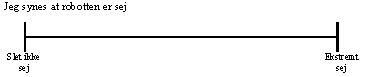
\includegraphics[width =\textwidth]{Figure/UdvalgteSkalaer/SejR} 
\caption{Unipolær VAS med lukkede endepunkter til skala spørgsmålet: \textit{Jeg synes at robotten er sej}.}
\label{fig:SkalaSejR}
\end{figure}
\noindent
%
Tilsvarende gør sig gældende for hvorhvidt robotten er sej. 
%
\begin{figure}[H]
\centering
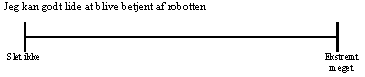
\includegraphics[width =\textwidth]{Figure/UdvalgteSkalaer/BetjeningAfR} 
\caption{Unipolær VAS med lukkede endepunkter til skala spørgsmålet: \textit{Jeg kan godt lide at blive betjent af robotten}.}
\label{fig:SkalaBetjeningAfR}
\end{figure}
\noindent
%
Det har ikke været muligt at formulere skala spørgsmålet: \textit{Jeg kan godt lide at blive betjent af robotten} på en måde, hvorpå det ville give mening at præsentere spørgsmålet på en bipolær skala, hvorfor det e præsenteres på en unipolær skala.\blankline
%
Det vælges at medtage de to potentielle skala spørgsmål til kategorien: \textit{Kendskab til teknologi}. Det første skala spørgsmål vedrører hvordan det var at interagere med robotten, \autoref{fig:SkalaHvordanVarDetAtBrugeR}, og det andet handler om ens kendskab til teknologi, \autoref{fig:AFKendskabTilTeknologi}.
%
\begin{figure}[H]
\centering
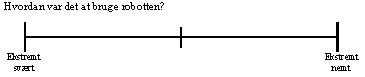
\includegraphics[width =\textwidth]{Figure/UdvalgteSkalaer/HvordanVarDetAtBrugeR} 
\caption{Bipolær VAS med lukkede endepunkter og unavngivet midtpunkt til skala spørgsmålet: \textit{Hvordan var det at bruge robotten?}}
\label{fig:SkalaHvordanVarDetAtBrugeR}
\end{figure}
\noindent
%
Det vurderes at \textit{nemt} og \textit{svært} er hinandens modpart, hvorfor de anvendes som labels på endepunkterne. Dog har det ikke været muligt, at finde et naturligt og logisk label til midtpunktet. 
%
\begin{figure}[H]
\centering
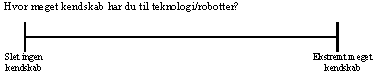
\includegraphics[width =\textwidth]{Figure/UdvalgteSkalaer/KendskabTilTeknologi} 
\caption{Unipolær VAS med lukkede endepunkter til skala spørgsmålet: \textit{Hvor meget kendskab har du til teknologi/robotter?}}
\label{fig:SkalaKendskabTilTeknologi}
\end{figure}
\noindent
%
Dette skala spørgsmål medtages men det vil indgå som en del af demografi, hvorfor det ikke vil indgå samme med de andre skalaer. Årsagen til at det overhovedet inkluderes er, at det forventes, at ens kendskab til teknologi har indflydelse på hvordan HRI evalueres. Dog er det ikke besluttet om skala spørgsmålet skal vedrører ens kendskab til teknologi eller ens kendskab til robotter. \blankline 
%
De tre potentielle skala spørgsmål fra kategorien: \textit{Tillid til R} medtages. På den første skala skal testpersonen angive hvor forskrækket robotten gjorde en, jævnfør \autoref{fig:SkalaForskraekket}, hvor på den næste evaluerer testpersonen hvorvidt de regnede med at robotten fulgte dem hen til det valgte sted, jævnfør \autoref{fig:SkalaRFulgteMigDetRigtigeStedHen}, og på den sidste skala evaluerer testpersonen hvor tryg de er ved robotten, jævnfør \autoref{fig:SkalaTrygVedR}.
%
\begin{figure}[H]
\centering
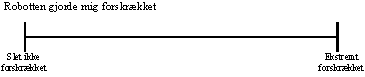
\includegraphics[width =\textwidth]{Figure/UdvalgteSkalaer/Forskraekket} 
\caption{Unipolær VAS med lukkede endepunkter til skala spørgsmålet: \textit{Robotten gjorde mig forskrækket}.}
\label{fig:SkalaForskraekket}
\end{figure}
\noindent
%
Da der ikke kunne findes en naturlig og logisk modpart til forskrækket vælges det, at præsentere skala spørgsmålet på en unipolær skala, jævnfør \autoref{fig:SkalaForskraekket}. 
%
\begin{figure}[H]
\centering
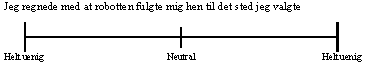
\includegraphics[width =\textwidth]{Figure/UdvalgteSkalaer/RobottenFulgteMigDetRigtigeStedHen} 
\caption{Bipolær VAS med lukkede endepunkter og navngivet midtpunkt til skala spørgsmålet: \textit{Jeg regnede med at robotten fulgte mig hen til det sted jeg valgte}.}
\label{fig:SkalaRFulgteMigDetRigtigeStedHen}
\end{figure}
\noindent
%
Da skala spørgsmålet på \autoref{fig:SkalaRFulgteMigDetRigtigeStedHen} er formuleret som det er, afspejler det i højere grad et udsagn en testperson kan erklærer sig enig eller uenig i, fremfor at testpersonerne angiver hvor meget de oplever en bestemt parameter. Derudover vurderes det at der findes et naturligt og logisk midtpunkt mellem at være \textit{helt uenig} og \textit{helt enig} nemlig \textit{neutral}.  
%
\begin{figure}[H]
\centering
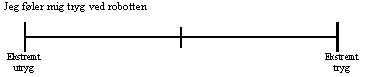
\includegraphics[width =\textwidth]{Figure/UdvalgteSkalaer/TrygVedR} 
\caption{Bipolær VAS med lukkede endepunkter og unavngivet midtpunkt til skala spørgsmålet: \textit{Jeg føler mig tryg ved robotten}.}
\label{fig:SkalaTrygVedR}
\end{figure}
\noindent
%
Årsagen til at der ikke er et label på skalaens midtpunkt er, at der ikke forekommer et bestemt ord, som er en naturlig og logisk midte mellem \textit{ekstremt utryg} og \textit{ekstremt tryg}. Derudover vurderes det at markeringen af midtpunktet i sig selv bør være nok til at forstå skala.\blankline
%
Ud af de 30 potentielle skala spørgsmål til de ti kategorier præsenteret i \fullref{ParametreDatabehandlingAffinityDiagram} er der nu udvalgt og opstillet 24 skalaer, som ud fra projektgruppens vurdering kan anvendes til at evaluere HRI. Hver skala afspejler en specifik parameter, som bygger på de danske rejsendes udtalelser omkring mødet med robotten i Aalborg Lufthavn.     
